\documentclass[9pt]{article} 

\usepackage{amsmath, amssymb, graphicx}
\usepackage{titlesec}
\usepackage{lipsum}  
\usepackage{xcolor}
\usepackage{titlesec} 
\usepackage{graphicx} 
\usepackage{pgfplots}
\usepackage{pgfplotstable} 
\pgfplotsset{compat=1.17} 
\usepackage{tikz}
\usepackage[export]{adjustbox}
\usepackage{geometry}
\usepackage{mdframed}
\usepackage{amsmath}
\usepackage{hyperref}
\geometry{a4paper, left=2cm, right=2cm, top=2cm, bottom=2cm}

% traitement du langage python:
\usepackage{listings}
\usepackage{color}

\definecolor{codegreen}{rgb}{0,0.6,0}
\definecolor{codegray}{rgb}{0.5,0.5,0.5}
\definecolor{codepurple}{rgb}{0.58,0,0.82}
\definecolor{backcolour}{rgb}{0.95,0.95,0.92}

\lstdefinestyle{mystyle}{
    backgroundcolor=\color{backcolour},
    commentstyle=\color{codegreen},
    keywordstyle=\color{magenta},
    numberstyle=\tiny\color{codegray},
    stringstyle=\color{codepurple},
    basicstyle=\ttfamily\small,
    breakatwhitespace=false,
    breaklines=true,
    captionpos=b,
    keepspaces=true,
    numbers=left,
    numbersep=5pt,
    showspaces=false,
    showstringspaces=false,
    showtabs=false,
    tabsize=2
}

\lstset{style=mystyle}
% fin traitement du langage python

\definecolor{section}{RGB}{0, 102, 153}
\definecolor{sub_section}{RGB}{128, 0, 32}
\definecolor{important}{RGB}{0, 128, 64}      
\definecolor{info}{RGB}{255, 255, 204}  

\title{Titanic - Machine Learning from Disaster}
\author{CHARLEMAGNE Clément}
\date{\today} 

\titleformat{\section}{\normalfont\Large\bfseries}{\thesection}{1em}{}
\titleformat{\subsection}{\normalfont\large\bfseries}{\thesubsection}{1em}{}
\titleformat{\subsubsection}[runin]{\normalfont\normalsize\bfseries}{\thesubsubsection}{1em}{}[:]

\begin{document}

\maketitle

\begin{center}
    
\includegraphics[width=\linewidth]{/home/charlemagne/workspace/kaggle_challenge_titanic/img/header.jpeg}
\end{center}

\vspace*{100pt}

\begin{center}
    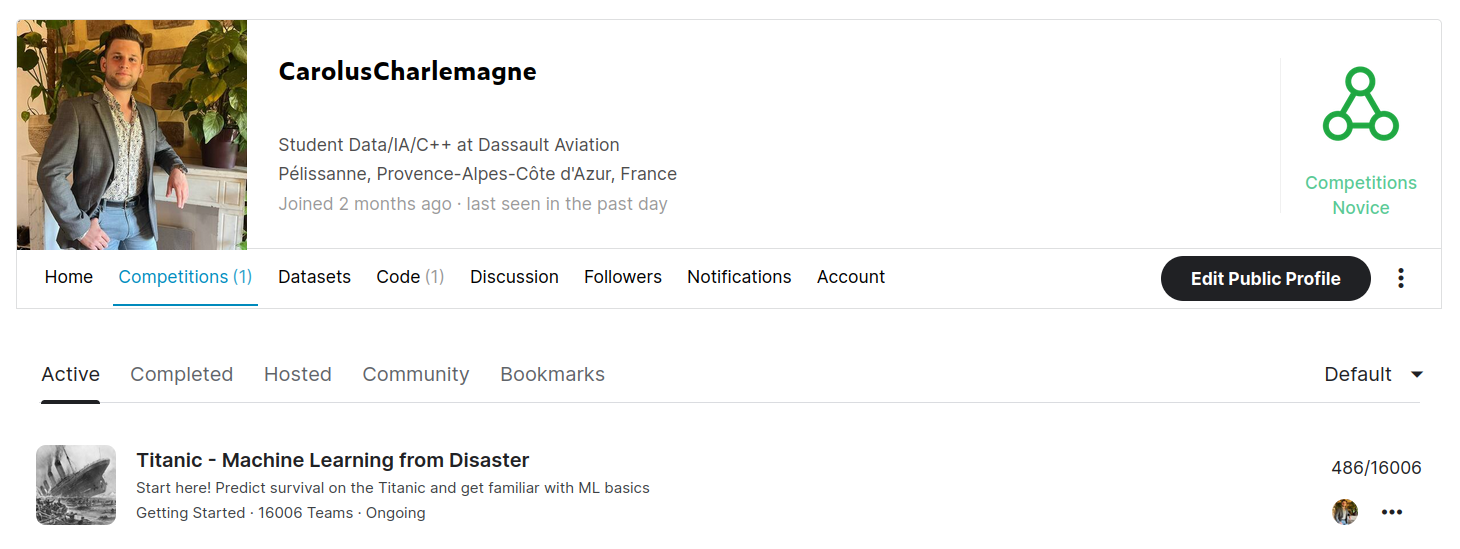
\includegraphics[width=\linewidth]{/home/charlemagne/workspace/kaggle_challenge_titanic/img/position.png}
\end{center}

\clearpage
\section{\textcolor{section}{Analyse des données et prétraitement}}

\begin{figure}[htbp]
    \centering
    \begin{minipage}{0.45\textwidth}
        \centering
        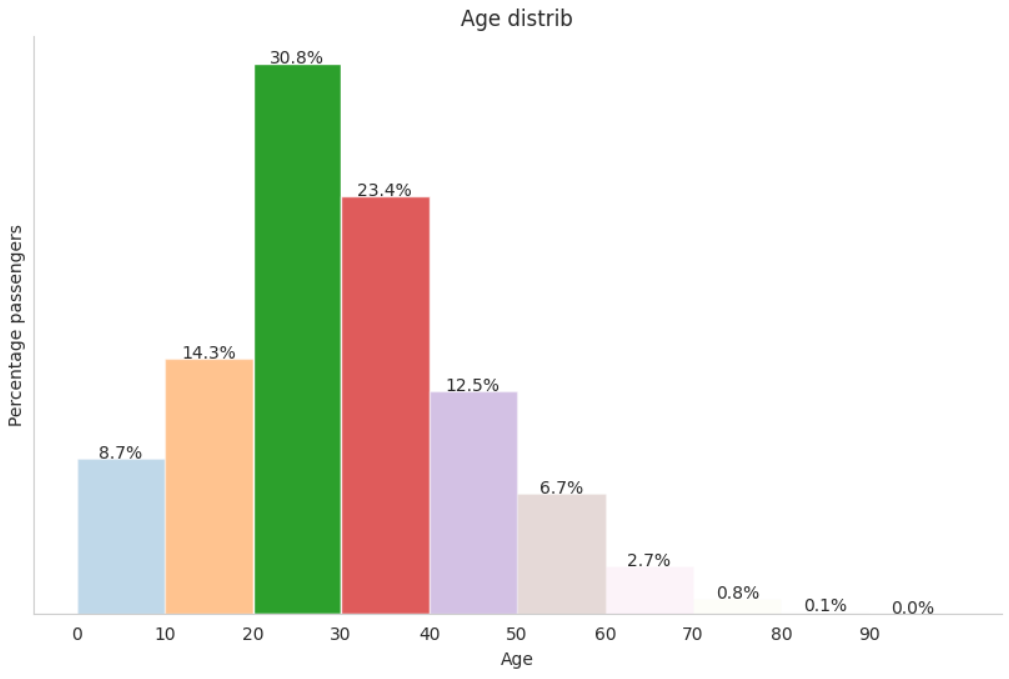
\includegraphics[width=\linewidth]{/home/charlemagne/workspace/kaggle_challenge_titanic/img/distrib_age.png}
    \end{minipage}\hfill
    \begin{minipage}{0.45\textwidth}
        J'ai commencé par réaliser un graphique simpliste, permettant de se concentrer sur l'essentiel.
         Chaque barre représente une tranche d'âge de 10 ans et la hauteur de la barre indique le pourcentage 
         de passagers qui se situent dans cette tranche d'âge. Les valeurs null ont été exclues. Plus un décile
          est représenté dans les données, moins la couleur de celle-ci est opaque. Nous permettant de voir dès 
          le premier coup d'oeil que la plage 20/30 ans est la plus représentée.
    \end{minipage}
\end{figure}

\begin{figure}[htbp]
    \centering
    \begin{adjustbox}{width=0.80\linewidth}
    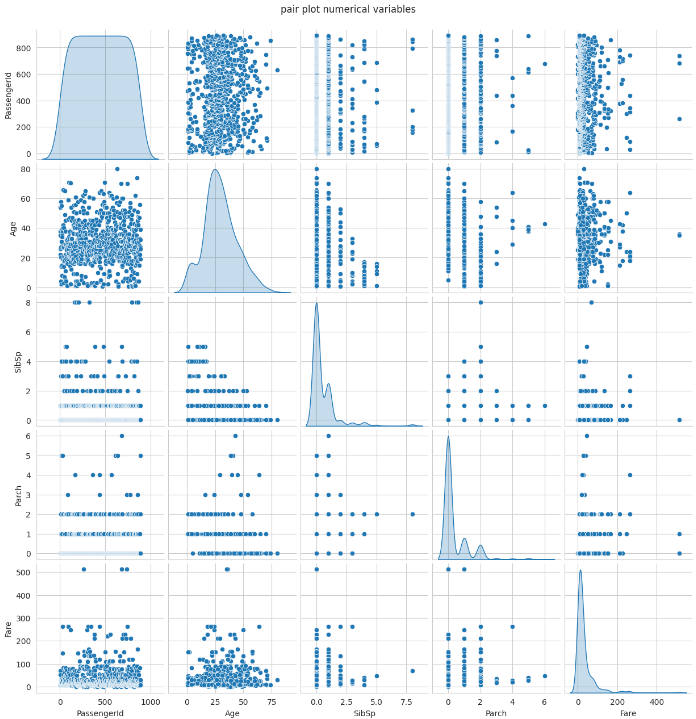
\includegraphics[width=1\linewidth, angle=0]{/home/charlemagne/workspace/kaggle_challenge_titanic/img/matrice_dispersion_quantitatives.png}
    \end{adjustbox}
\end{figure}
\noindent J'ai ensuite réalisé une matrice de dispersion des variables quantitatives du jeu de données, m'ayant permis de remarquer
les points suivants:
\begin{itemize}
    \item Beaucoup de jeunes passagers.
    \item Très peu de passagers avec des frères et soeurs ou des conjoints.
    \item Peu de passagers avec leurs parents ou enfants.
    \item La majorité des billets vendus étaient à bas prix.
    \item Il semblerait que les billets aux prix les plus élevés, ont été vendus aux personnes
    plus agées en moyenne.
\end{itemize}

\clearpage
\begin{figure}[htbp]
    \centering
    \begin{adjustbox}{width=1\linewidth}
    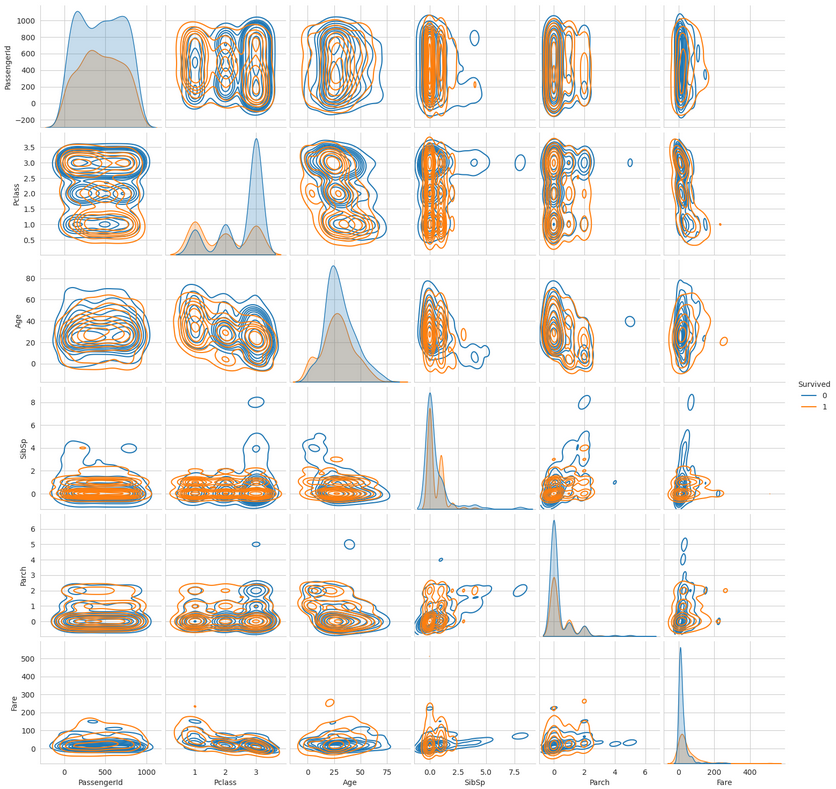
\includegraphics[width=1\linewidth, angle=0]{/home/charlemagne/workspace/kaggle_challenge_titanic/img/matrice_dispersion_survie_v2.png}
    \end{adjustbox}
\end{figure}
\noindent J'ai ensuite réalisé une matrice de dispersion colorée par la variable catégorielle Survided, m'ayant permis de remarquer
les points suivants:
\begin{itemize}
    \item Les passagers de première classe avaient de meilleurs chances de survie.
    \item D'avantage de suivants parmis les enfants.
    \item Les familles de 2 ou 3 personnes ont plus de chances de survie que les familles plus 
    nombreuses ou les personnes seules.
\end{itemize}

\vspace*{12pt}

\noindent Le code ci-dessous, dédié au prétraitement des données réalise les étapes suivantes:
\begin{itemize}
    \item Normalisation des noms (retire les points, sépare les noms par des espaces).
    \item Extraction du numéro de billet et séparation des élémentrs, retourne NONE si un seul élément est
    trouvé.
    \item Utilisation de Tensorflow pour la tokenization.
    \item Conversion des dataframes en datasets TensorFlow avec la colonne Survived comme label.
    \item Suppresion de certaines colonnes pour ne pas les utiliser comme caractéristiques d'apprentissage
    du modèle(PassengerId car inutile et Survided car sert déjà de label).
\end{itemize}
\begin{lstlisting}[language=Python, caption={Traitement des données}]
def preprocess(df):
df = df.copy()

def normalize_name(x):
    return " ".join([v.strip(",()[].\"'") for v in x.split(" ")])

def ticket_number(x):
    return x.split(" ")[-1]
    
def ticket_item(x):
    items = x.split(" ")
    if len(items) == 1:
        return "NONE"
    return "_".join(items[:-1])

df["Name"] = df["Name"].apply(normalize_name)
df["Ticket_number"] = df["Ticket"].apply(ticket_number)
df["Ticket_item"] = df["Ticket"].apply(ticket_item)
return df

def tokenize_names(features, labels=None):
features["Name"] = tf.strings.split(features["Name"])
return features, labels

preprocessed_train_df = preprocess(train_df)
preprocessed_test_df = preprocess(test_df)

input_features = list(preprocessed_train_df.columns)
input_features.remove("Ticket")
input_features.remove("PassengerId")
input_features.remove("Survived")

train_ds = tfdf.keras.pd_dataframe_to_tf_dataset(preprocessed_train_df, label="Survived").map(tokenize_names)
serving_ds = tfdf.keras.pd_dataframe_to_tf_dataset(preprocessed_test_df).map(tokenize_names)
\end{lstlisting}



\clearpage
\section{\textcolor{section}{Choix du modèle et analyse des résultats}}
\begin{lstlisting}[language=Python, caption={Traitement des données}]
def prediction_to_kaggle_format(model, threshold=0.5):
proba_survive = model.predict(serving_ds, verbose=0)[:, 0]
return pd.DataFrame({
    "PassengerId": preprocessed_test_df["PassengerId"],
    "Survived": (proba_survive >= threshold).astype(int)
})

num_trees = 300
min_examples = 5
categorical_algorithm = "CART"

model = tfdf.keras.GradientBoostedTreesModel(
    verbose=0,
    features=[tfdf.keras.FeatureUsage(name=n) for n in input_features],
    exclude_non_specified_features=True,
    random_seed=1234,
    num_trees=num_trees,
    min_examples=min_examples,
    categorical_algorithm=categorical_algorithm
)
model.fit(train_ds)
\end{lstlisting}

\noindent Le code ci-dessus présente l'utilisation du modèle GBT, pour Gradient Boosted Trees, un modèle
puissant et robuste face aux différentes échelles et types de données. Le nombre d'arbres est de 300, plus il 
y a d'arbres, plus le modèle est puissant. Cependant, plus le nombre d'arbres  augmente, plus le modèle risque 
de trop s'ajuster aux données. En voulant augmenter le nombre d'arbres, j'ai fais passer mon score Kaggle de 0.80382
à moins de 0.7\dots \\
J'ai utilisé l'algorithme CART pour sa grand flexibilité, ses performances en classification et régression, ainsi que sa 
facilité d'interprétation. 
J'ai utilisé pour mon premier script "dumb", un modèle random forest assez basique, avec les bons réglages j'ai pu obtenir un score 
de 0.75 sur Kaggle, me plaçant dans les 12 000 premiers. Une fois ce modèle testé, j'ai regardé ce qu'il été commun de faire pour 
s'améliorer dans ce challenge, je me suis aperçu que des arbres de décisions ou des GBT permettaient d'obtenir de très bons scores
(entre 0.8 et 0.9). J'ai en effet obtenu mes meilleurs résultats avec GBT, dans mon cas, meme XGB n'a pas su faire mieux\dots \\
Je suis persuadé qu'avec un meilleur prétraitement des données, comme dans cet exemple \\
(https://www.kaggle.com/code/vbmokin/titanic-top-3-cluster-analysis/notebook), et le modèle GBT, nous\\ 
pourrions faire un meilleur score

\end{document}




\href[pdfnewwindow=true]{https://imbalanced-learn.org/stable/over_sampling.html#from-random-over-sampling-to-smote-and-adasyn}{Illustration de ces méthodes de ré-échantillionage.}

\paragraph[short]{}{}

\begin{mdframed}[backgroundcolor=info] \end{mdframed}    

\begin{lstlisting}[language=Python, caption={}]\end{lstlisting}

\texttt{dataframe.drop\_duplicates()}

\begin{figure}[htbp]
    \centering
    \begin{adjustbox}{width=1\linewidth}
    \includegraphics[width=1\linewidth, angle=0]{/home/charlemagne/workspace/data_ia_perso/img/data_science/histogramme_ditribution_poids_diff_bin_python.png}
    \end{adjustbox}
\end{figure}

\clearpage